\documentclass[a2paper, 12pt]{article}
\usepackage[font={huge, bf}]{caption}
\usepackage{fontspec}
\setmainfont{Arial}
\usepackage{subcaption}
\usepackage{graphicx}
\usepackage{tikz}
\usepackage{tikzsymbols}
\usetikzlibrary{calc,patterns,shapes.geometric}
\usepackage{float}
\usepackage{pdflscape}
\usepackage{geometry}
\geometry{landscape, margin=2cm}
\captionsetup[subfigure]{justification=justified,singlelinecheck=false}
\pagestyle{empty}

\def\centerarc[#1](#2)(#3:#4:#5){\draw[#1] ($(#2)+({#5*cos(#3)},{#5*sin(#3)})$) arc (#3:#4:#5);}

\begin{document}
	\vspace*{\fill}
	\begin{figure}[!htbp]
		\centering
		\begin{subfigure}[b]{0.48\textwidth}
			\caption{Figure 1}
			\centering
			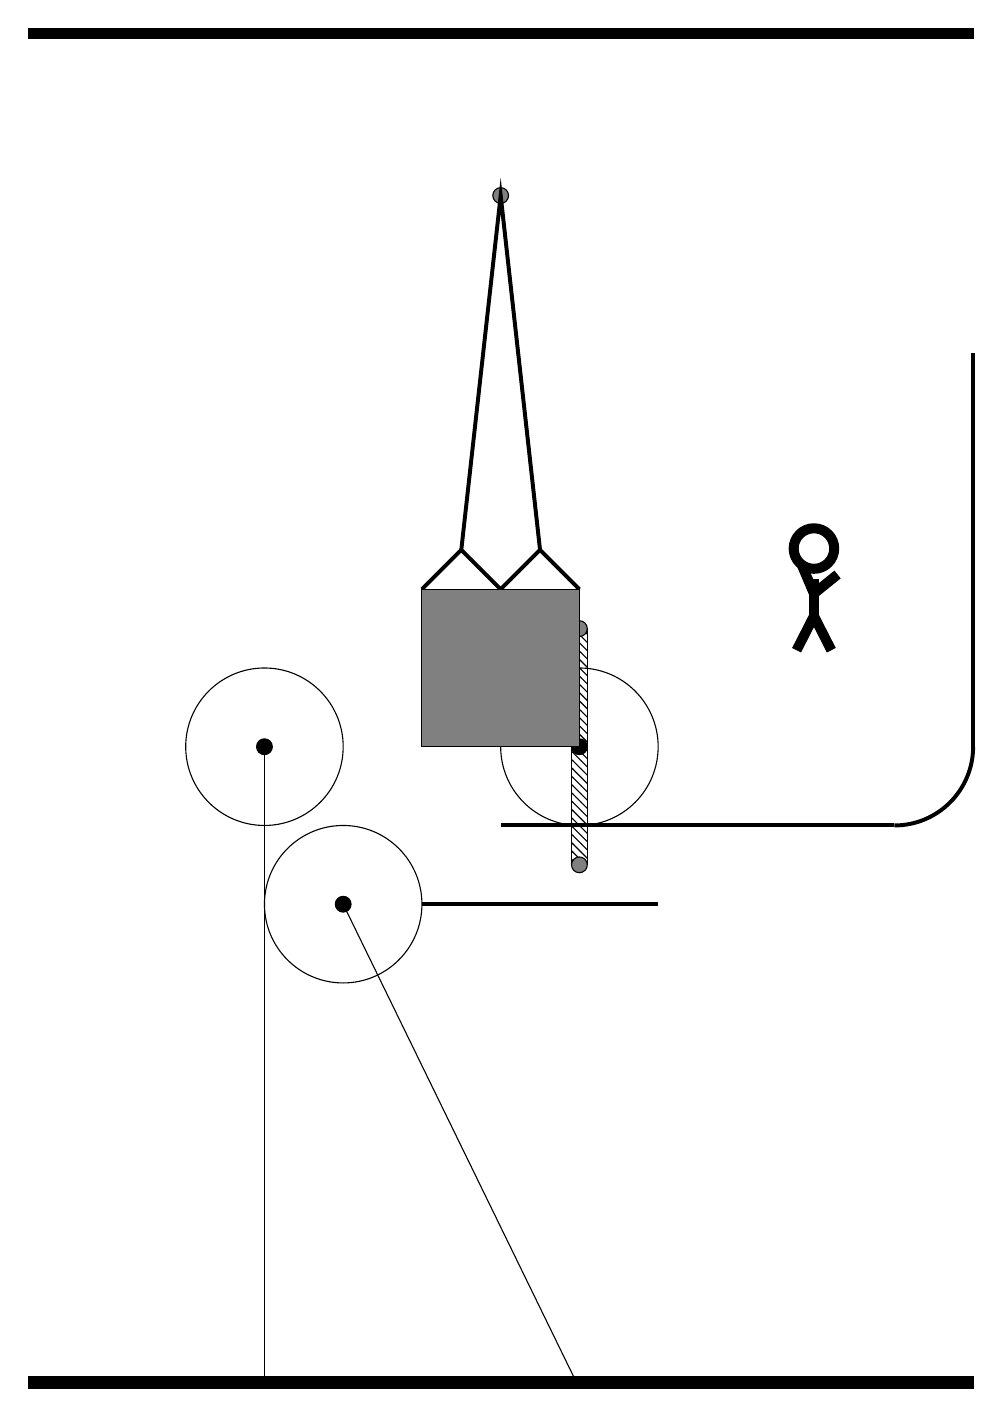
\begin{tikzpicture}
				\draw[fill=black] (-2, 14) rectangle (10, 14.125);
				
				\draw (1,5) circle (1);
				\draw[fill=black] (1,5) circle (0.1);
				\draw (1,-3.15) -- (1,5);
				
				\draw (5,5) circle (1);
				\draw[fill=black] (5,5) circle (0.1);
				\draw[pattern=north west lines, pattern color=black] (4.9,6.5) rectangle (5.1,3.5);
				\draw[fill=black!50] (5,6.5) circle (0.1);
				\draw[fill=black!50] (5,3.5) circle (0.1);
				
				\draw (2,3) circle (1);
				\draw[fill=black] (2,3) circle (0.1);
				\draw (5,-3.15) -- (2,3);
				
				\draw[fill=black!50] (4,12) circle (0.1);
				\draw[line width=0.5mm](3.5,7.5) -- (4,12) --  (4.5,7.5);
				\draw[line width=0.5mm](3,7) --  (3.5,7.5) -- (4,7) -- (4.5,7.5) -- (5,7);
				\draw[fill=black!50] (3, 7) rectangle (5, 5);
				
				\draw[line width = 0.5mm] (4,4) -- (9,4);
				\draw[line width = 0.5mm] (9,4) arc (270:360:1);
				\draw[line width = 0.5mm] (10,5) -- (10,10);
				\draw[line width = 0.5mm] (3,3) -- (6,3);
				
				\node at (8, 7) {\scriptsize \Strichmaxerl[10][-67][39]};
				
				\draw[fill=black] (-2, -3) rectangle (10, -3.15);
			\end{tikzpicture}
		\end{subfigure}
		\hfill
		\begin{subfigure}[b]{0.48\textwidth}
			\caption{Figure 2}
			\centering
			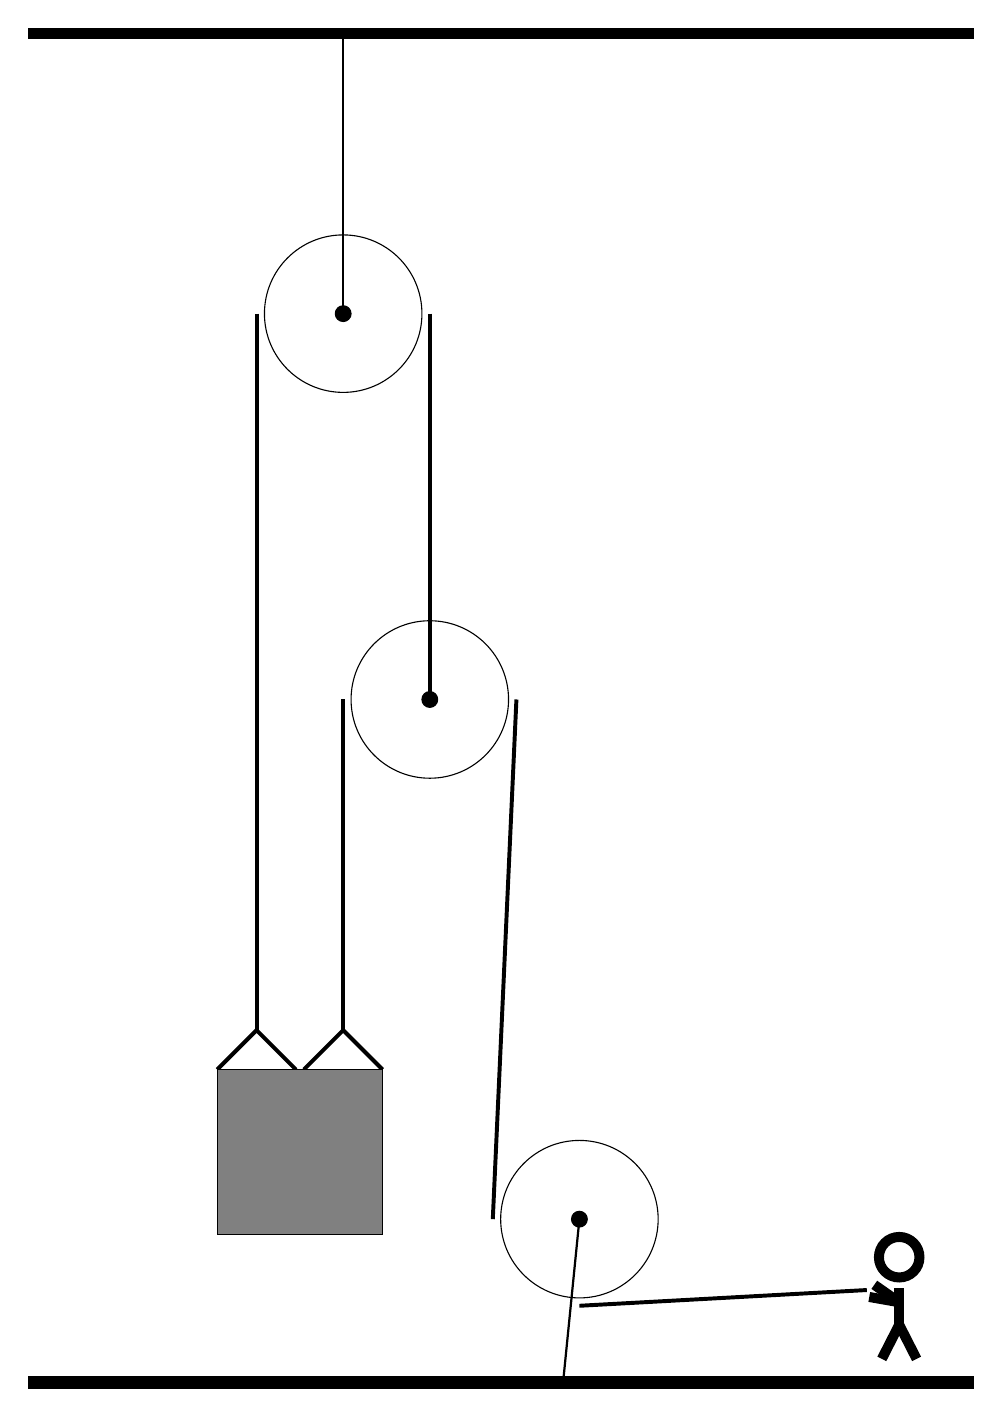
\begin{tikzpicture}
				\draw[fill=black] (-2, 14) rectangle (10, 14.125);
				
				\draw (2, 10.5) circle (1);
				\draw[fill=black] (2, 10.5) circle (0.1);
				\draw[thick] (2, 10.5) -- (2, 14);
				
				\draw (3.1, 5.6) circle (1);
				\draw[fill=black] (3.1, 5.6) circle (0.1);
				
				\draw (5, -1) circle (1);
				\draw[fill=black] (5, -1) circle (0.1);
				\draw[thick] (5, -1) -- (4.8, -3);
				
				\draw[line width = 0.5mm]  (0.4, 0.9) -- (0.9, 1.4) -- (1.4, 0.9);
				\draw[line width = 0.5mm]  (1.5, 0.9) -- (2.0, 1.4) -- (2.5, 0.9);
				\draw[fill=black!50] (0.4, 0.9) rectangle (2.5, -1.2);
				
				\draw[line width = 0.5mm] (0.9, 10.5) -- (0.9, 1.4);
				\centerarc[line width = 0.5mm](2, 10.5)(0:180:1.1);
				\draw[line width = 0.5mm] (3.1, 10.5) -- (3.1, 5.6);
				\draw[line width = 0.5mm] (2.0, 5.6) -- (2.0, 1.4);
				\centerarc[line width = 0.5mm](3.1, 5.6)(0:180:1.1);
				\draw[line width = 0.5mm] (4.2, 5.6) -- (3.9, -1);
				\centerarc[line width = 0.5mm](5, -1)(180:270:1.1);
				\draw[line width = 0.5mm] (5, -2.1) -- (8.65, -1.9);
				
				\node at (9, -2) {\scriptsize \Strichmaxerl[10][-35][170]};
				
				\draw[fill=black] (-2, -3) rectangle (10, -3.15);
			\end{tikzpicture}
		\end{subfigure}
	\end{figure}
		\vspace*{\fill}
\end{document}